\usetikzlibrary{calc}
\usetikzlibrary{positioning}
\usetikzlibrary{matrix}
\usetikzlibrary{mindmap,trees,shapes,snakes}

\chapterimage{chapter_head_1.png}

\chapter{Objekterkennung und Computer Vision}
\section{Intro \& Motivation}
Wie können wir uns eigentlich in der Welt, in der wir sind, zurechtfinden? Die \textbf{Wahrnehmung} ermöglicht die Aufnahme von Informationen über die Umgebung. Der Menschen hat fünf Hauptwahrnehmungssinne: Sehen, Hören, Tasten, Riechen und Schmecken. Können wir einer künstlichen Intelligenz (KI) diese Wahrnehmung beibringen? Wenn ja, wie?

Sinne bei KIs nennen wir \textbf{Sensoren}. Solche, die wir in KIs einbauen können, sind Sehen, Hören und Tasten. \textbf{Sehen} ist dabei im Hinblick auf den Gebrauch von KIs in der physischen Welt für uns Menschen der hilfreichste von allen.

In dieser Ausarbeitung werden zunächste Grundlagen über die Funktionsweise des Sehens beschrieben. Der Fokus wird dann auf die Verarbeitung von gewonnenen Rohinformationen liegen und ein paar Anwendungen ansprechen.

\section{Überblick Computer Vision}
Die Frage die Computer Vision stellt, ist eigentlich recht einfach: Wenn ein von der Umgebung ausgelöster Sensor-Impuls (S) so und so aussieht, wie sieht dann die Umgebung (W) dazu aus? Leider ist das Invertieren dieser Funktion
\begin{equation*}
S = f(W) \Rightarrow W = f^{-1}(S)
\end{equation*}
nicht so einfach möglich. Man muss sich also überlegen, anhand welcher Merkmale Entscheidungen über den Inhalt eines Bildes getroffen werden können. Computer Vision lässt sich dafür grob in drei Stufen einteilen:
\begin{itemize}
\item \textit{Low-Level Vision}: Grundlegende Untersuchung des Bildes auf herausstechende Features wie Unterschiede in Helligkeit, Farben oder Texturen und die damit verbundene Kantendetektion
\item \textit{Medium-Level Vision}: Objekterkennung und Bewegungsanalyse mithilfe der zuvor gesammelten Informationen
\item \textit{High-Level Vision}: Die Kombination und Analyse aller Daten: Was sagt mir das Bild, wie reagiere ich darauf?
\end{itemize}

Die Hauptanwendungsgebiete hierfür sind:
\begin{itemize}
\item Manipulation: Die Erlangung von benötigen Informationen von und Rückmeldung über lokale Gebilde, um mit diesen zu interagieren (z.~B.\ greifen, einfügen; Anwendung: z.~B.\ Qualitätskontrolle).
\item Navigation: Die Berechnung der eigenen Geschwindigkeit und Position (Ausrichtung), um Routen zu planen und Hindernissen auszuweichen.
\item Objekterkennung: Die Charakterisierung von Objekten zur Unterscheidung von \glqq gut\grqq\ und \glqq schlecht\grqq\ (z.~B.\ Beute- und Raubtier, (un)genie"sbare Früchte, Bekannte und Fremde).
\end{itemize}

Wir werden uns hier nur mit Low-Level- und Medium-Level Vision beschäftigen.
Zunächst werden wir auf die Entstehung von Bildern, Bildverarbeitungsoperationen, nutzbare Hinweise in Bildern, optisch gesteuerte Manipulation und Navigation und schließlich verschiedene Ansätze zur Objekterkennung eingehen.

\subsection{Grundlagen der Bildentstehung}

Um Informationen über einen \textbf{Ort} zu erhalten, benötigen wir ein Bild. Um ein \textbf{Bild} (2D) zu erstellen, müssen wir \textbf{Sehen} (3D) können. Das Sehen, so wie es in unseren Augen passiert, ist sehr komplex. Vereinfacht können wir es jedoch  anhand einer Lochkamera erkl"aren - der Prozess ist ungef"ahr der Gleiche.

\subsubsection{Lochkamera}

\marginpar[Links]{\small{(wer mit diesem Prinzip bereits vertraut ist, kann die nächste Seite überspringen)}}

\begin{figure}[h]
\centering
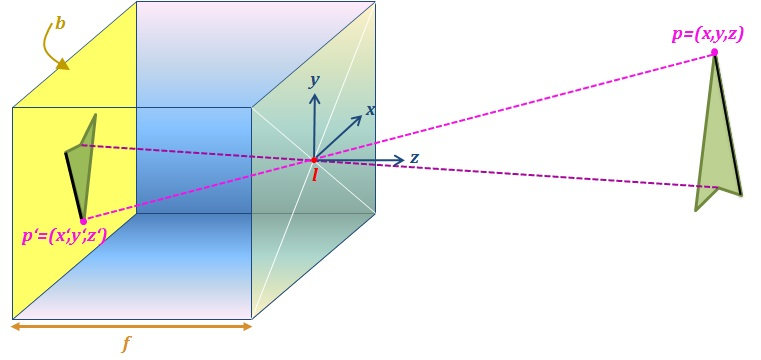
\includegraphics[width=8cm]{chapters/computervision/Grafik_1_Lochkamera.JPG}
\caption{Geometrie der Bildentstehung in einer Lochkamera.}
\label{fig:1}
\end{figure}
Eine Lochkamera ist eine schwarze Box, die an ihrer Front nur durch einen Punkt Licht eindringen lässt, welcher auf die Bildebene (Wand parallel zur Front) trifft. Je nachdem, wie gro"s die Lochblende ist, gelangen weniger oder mehr Lichtstrahlen hindurch. Je kleiner das Loch ist, desto schärfer ist das Bild, vor allem bei Objekten, die einen kleinen Abstand zur Lochkamera haben. Sobald das Loch vergrö"sert wird, gelangen mehr Lichtstrahlen hindurch, also wird ein Punkt vom Objekt durch mehrere Lichtstrahlen auf die Bildebene geschickt und das Bild erscheint uns unscharf.
\begin{figure} [h]
\centering
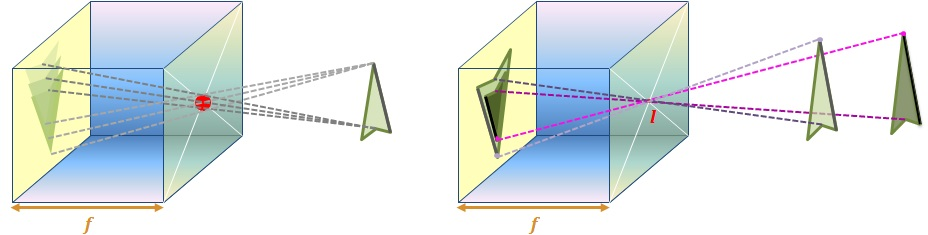
\includegraphics[width=12cm]{chapters/computervision/Grafik_3_Lochkamera.JPG}
\caption{Größe der Lochblende beeinflusst die Schärfe (links), der Abstand vor der Lochblende beeinflusst die Projektionsgrö"se (rechts).}
\label{fig:3}
\end{figure}

Wir betrachten einen Punkt $p$ mit den Koordination $(x,y,z)$ und seine \glqq Kopie\grqq\ $p'=(x',y',z')$ auf der Bildebene. $f$ beschreibt den Abstand zwischen der Lochblende $l$ und der Bildebene $b$.
\begin{figure}[h]
\centering
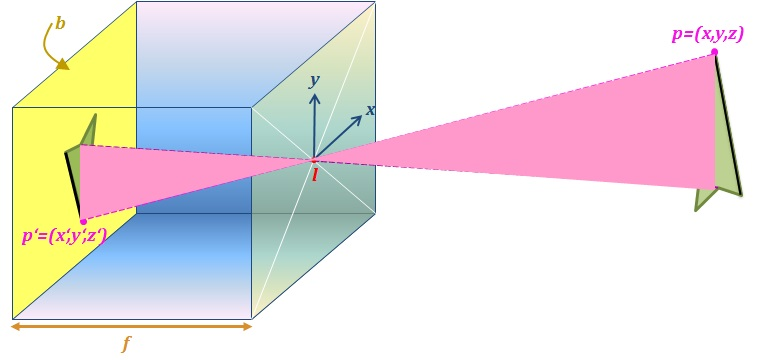
\includegraphics[width=8cm]{chapters/computervision/Grafik_2_Lochkamera.JPG}
\caption{Invertierte, gleiche Dreiecke.}
\label{fig:2}
\end{figure}
Es entstehen zwei kongruente Dreiecke, sodass wir die folgenden Umformungen vornehmen können:
\[\frac{-x'}{f}=\frac{x}{z},\quad \frac{-y'}{f}=\frac{y}{z} \quad \Rightarrow \quad x'=\frac{-fx}{z}, \quad y'=\frac{-fy}{z}\]
Wie auf der Abbildung zu sehen ist, wird das Objekt auf der Bildebene invertiert, sodass das Objekt sowohl auf dem Kopf steht als auch gespiegelt ist (in der Gleichung ist dieser Vorgang durch das negative Vorzeichen markiert). Was hier passiert hei"st \textbf{perspektivische Projektion}: parallele Linien treffen sich in einem \textbf{Fluchtpunkt} in der Ferne. Hierfür ist ausschlie"slich der Richtungsvektor der Linien ausschlaggebend.
Für eine Linie mit der Richtung $(u,v,w)$, die durch einen Punkt $p=(x,y,z)$ geht, gilt, dass die Projektion $P_\lambda$ auf der Bildebene für jeden Punkt $p'=(x+\lambda u,y+\lambda v,z+\lambda w)$ mit $\lambda\in (-\infty,+\infty)$ auf ihr durch
\[P_\lambda=\Bigg( f\frac{x+\lambda u}{z+\lambda w},f\frac{v+\lambda v}{z+\lambda w} \Bigg)\]
gegeben ist.

\subsubsection{Linsensysteme}
Linsen sind dem menschlichen Auge nachempfunden und im Vergleich zu Lochblenden viel grö"ser, sodass mehr Licht hindurch gelangt. Dadurch können nicht alle Objekte der Welt gleichzeitig scharf auf der Bildebene abgebildet werden, sondern nur solche, die sich im Bereich der \textbf{Tiefenschärfe} - also in einem bestimmten Abstand zur Linse - befinden.

In der Linse werden alle von einem Objekt eingehenden Strahlen so gebrochen, dass sie sich in einem Punkt hinter der Linse schneiden.
Die \textbf{Brennweite} $f$ der Linse, bei der ein bestimmtes Objekt scharf dargestellt wird, ergibt sich aus den Punkten $z$ (Abstand des Objekts zur Linse) und $z'$ (Abstand von der Linse zur Bildebene). Die Beziehung zwischen $z$ und $z'$ wird mit
\[\frac{1}{z}+\frac{1}{z'}=\frac{1}{f}\]
beschrieben. Da $z$ überwiegend sehr viel grö"ser als $z'$ ist, wird die Abschätzung
\[\frac{1}{z}+\frac{1}{z'}\approx\frac{1}{z'}\quad\Rightarrow\quad\frac{1}{z'}\approx\frac{1}{f}\quad\Rightarrow z'\approx f.\]
gemacht.

\subsubsection{Licht und Schatten}

Typischerweise wird die Bildebene in einer Kamera mit einem Pixel-Raster der Grö"se $512\times 512$ bemessen. Die Bildhelligkeit über die Zeit wird durch $I(x,y,t)$ repräsentiert und kann modelliert werden. Sie ist von der vorhandenen Lichtmenge, der Objekt-Position und der Reflexionseigenschaften während der Bildaufnahme abhängig, wobei die Oberfläche des Objektes als auch die umliegenden Objekte Reflexionseigenschaften besitzen.
\begin{itemize}
\item
Wir sprechen von diffus reflektiertem Licht, wenn das Licht von der Objektoberfl"ache absorbiert und wieder abgestrahlt wurde, wodurch die Oberfl"ache von allen Richtungen aus gleich hell erscheint. Eine \textit{Lambert'sche} Ebene oder \emph{perfekter Streuk"orper} ist ein Objekt, das Licht vollst"andig diffus reflektiert. Ein perfekter Streukörper erzeugt die reflektierte Lichtintensität
$E = p\cdot E_0\cdot \mathrm{cos}\theta$
mit Lichtquelle $E_0$, Rückstrahlvermögen $p\in\lbrack 0,1\rbrack$ (schwarz bis wei"se Ebene) und $\theta$ zwischen der Richtung der Lichtquelle und der Oberfl"achennormale.
\item
Das spiegelnd reflektierte Licht hingegen wird "uberwiegend in eine bestimmte Richtung abgestrahlt. Der Reflexionswinkel stimmt hierbei mit dem Einfallswinkel überein, wie bei einer \textit{perfekten Spiegelreflexion}.
\item
Durch Unterschiede in der Lichtintensität entstehen \textbf{Schatten} auf Objekt-Oberflächen. Aus der gegebenen Helligkeit $I(x,y)$ unseres Bildes möchten wir auf die Geometrie und Reflexionseigenschaften der Umwelt schlie"sen. Für Oberflächen von Objekten können wir eine Reflexionskarte berechnen, welche ihre Reflexionseigenschaften beschreibt.
\end{itemize}
Bei der Computergrafik wird genau diese Lichtsituation, also die Welt um das Objekt, wo Licht aus verschiedenen Richtungen kommt und (mehrfach) reflektiert wird, versucht zu simulieren.
Normalerweise ist eine Mischung von direktem und indirektem Licht vorhanden. Wenn solche Interreflexion vorliegt, hilft uns die Reflexionskarte nicht weiter - ein Problem, welches noch nicht gelöst ist.

\subsubsection{Spektralphotometrie}

Neben dem Kontrastsehen gibt es noch das Farbsehen, welches sich in einem Wellenlängenbereich von Violett bis Rot, $400$nm--$700$nm, bewegt. Das menschliche Auge ist für drei verschiedene Spektralkurven empfindsam, sodass der unendlich-dimensionale Bereich der Wellenlänge auf einen drei-dimensionalen Farbbereich projiziert wird. So kommt es zu sogenannten \textbf{Metameren}: Verschiedene Lichtspektren, die von Menschen als gleiche Farben wahrgenommen werden.

\subsection{Bildverarbeitung und Bildhinweise - \glqq low-level\grqq}

Nun möchten wir ein aufgenommenes Bild analysieren und strukturieren.

Es gibt verschiedene Anhaltspunkte und Vorgehensweisen, mit denen wir 3D-Informationen verarbeiten können, um gewisse Aufgaben je nach Anwendungsgebiet (Manipulation, Navigation, Objekterkennung) zu lösen. In jedem Fall ziehen wir Informationen aus jedem \textbf{Pixel} (\textbf{pic}ture \textbf{el}ement = Bildpunkt). Dabei wird zwischen \textit{low-level} Wissen, beschränkt auf lokale Information von Pixeln, und \textit{high-level} Wissen, globale Information über Objekte, unterschieden.

Damit wir uns einen Überblick über unser Bild verschaffen können, ist es hilfreich, dieses zunächste in prägnante Bereiche zu unterteilen, also \textbf{Kanten} zu finden und \textbf{Regionen} zu identifizieren.

\subsubsection{Kantenermittlung}

Kanten entstehen durch Helligkeitsunterschiede. Wir unterscheiden verschiedene solcher \textbf{Diskontinutäten}: Tiefe, Oberfläche, Reflexion, Schatten.

Um Kanten zu finden, betrachten wir die Helligkeitsfunktion $I(x)$ und bilden ihre Ableitung $I'(x)$.
Dort wo die Steigung von $I'(x)$ gro"s ist, lässt sich eine Diskontinuität vermuten.
Jene Stellen, die nur kleinere Spitzen der Funktion sind, können durch \textbf{Rauschen} im Bild entstehen - also keine echten Kanten.
Dieses Rauschen k"onnen wir durch \textbf{Glättung} der Funktion eliminieren. Eine h"aufig verwendete Methode ist die \textbf{Faltung} von $I$ mit einer geeigneten Faltungsfunkton, etwa einer Gau"sschen Glockenkurve $G_\sigma$ oder ihrer Ableitung $G_\sigma'$. Dabei werden kleine Spitzen geglättet und gro"se Spitzen betont.

% TODO re-add images
%\begin{figure}[htbp]
%\centering
%\includegraphics[width=10cm]{Faltung_mit_Gauss_F.jpg}
%\caption{Helligkeitsfunktion $I(x)$ eines Bildes.}
%\label{fig:4}
%\includegraphics[width=10cm]{Faltung_mit_Gauss_Abl-F.jpg}
%\caption{Ableitung der Funktion $I'(x)$.}
%\label{fig:5}
%\includegraphics[width=10cm]{Faltung_mit_Gauss_F_G.jpg}
%\caption{Resultierende Funktion $I_G(x)=I*G'_\sigma$ durch Faltung.}
%\label{fig:6}
%\end{figure}

%In der entstehenden Funktion $I_G(x)$ lesen wir alle Spitzen ab, die oberhalb einer festgelegten Grenze (in Abb. \ref{fig:6} bspw. $0,5$) liegen, sodass Rauschen herausgefiltert wird.
% TODO: re-add reference to images
In der entstehenden Funktion $I_G(x)$ lesen wir alle Spitzen ab, die oberhalb einer festgelegten Grenze (bspw. $0,5$) liegen, sodass Rauschen herausgefiltert wird.


Die Tatsache, dass unsere Bildfunktion nicht ein- sondern zweidimensional ist,
macht den Vorgang technisch noch ein wenig komplexer, aber durch geeignete Rotation
der Faltungsfunktion kann man im Prinzip Punkte auf Kanten beliebiger Ausrichtung erkennen.
Kanten k"onnen wir nun als eine Reihe nebeneinanderliegender Kantenpunkte mit "ahnlichen Ausrichtungen identifizieren: Dies ist die Idee des sogenannten \textbf{Canny}-Kantenfinders.

\subsubsection{Segmentierung}

Jeder Pixel ist mit optischen Eigenschaften ausgestattet: Helligkeit, Farbe, Textur. Eine Region zeichnet sich dadurch aus, dass sich in ihr diese Eigenschaften nur geringfügig ändern.

Um Regionen zu identifizieren eignet sich die Kantenfindung vorerst schon, lässt aber dann zu wünschen übrig, wenn Kantenteile nicht (durch fehlenden Kontrast) oder aber fälschlicherweise (durch Rauschen, Oberflächenmarkierung, Schatten) erkannt werden. Es gibt zwei weitere Ansätze, welche die optischen Eigenschaften von Pixeln nutzen:

\begin{itemize}
\item \textit{Machine Learning} Ansatz [Malik]

Wir können eine Abgrenzungslinie $L$ finden, indem wir die Wahrscheinlichkeit $P_b(x,y,\theta)$ berechnen, dass $L$ durch einen Pixel $b=(x,y)$ mit dessen Orientierung $\theta$ verläuft.

Diese Methode funktioniert zwar besser, um Kanten im Bild zu finden, beschränkt sich aber auf den lokalen Kontext: Bestehende Regionen werden ggf.\ vernachlässigt, falls das Ende der Abgrenzungslinie $L$ nicht genau im Anfang mündet. Wenn also die Pixel auf $L$, zu sehr in ihren Eigenschaften variieren, wird $L$, die eine Region einkreist, nicht als \textit{eine} Linie erkannt und somit eben diese Region nicht als solche identifiziert.

\item \textit{Graph Partitioning} Ansatz (Shi und Malik, 2000)

In diesem Ansatz wird jeder Pixel als Knoten in einem Graph betrachtet. Kanten bestehen zwischen nebeneinanderliegenden Pixeln. Jede Kante wird mit einem Gewicht ausgestattet, welches die Ähnlichkeit der beiden Pixel in ihren optischen Eigenschaften repräsentiert.

Die Segmentierung besteht nun darin, den Graphen in Cluster zu zerteilen, sodass die Summe der Gewichte innerhalb einer Gruppe maximiert und zwischen den Gruppen minimiert wird.

%BILD ??

\end{itemize}

\subsection{Objekterkennung - \glqq high-level\grqq}

\subsubsection{Pose}

Die Position und Orientierung, die \textbf{Pose}, von Objekten, ist besonders für die Gebiete Manipulation und Navigation wichtig. Die Position eines Punktes ist seine Koordinate $P(x,y,z)$. Wir verfügen über dessen perspektivische Projektion auf unserem Bild mit der Koordinate $P'(x',y')$,
%(die Linie zwischen $P$ und $P'$ ist also der Lichtstrahl, der durch die Lochblende geht)%
kennen aber nicht die Entfernung von $P$ zur Kamera.

Wie können wir nun die Richtung des Objektes bestimmen? Entweder, wir betrachten das Objekt als ganzes (Koordinatensystem mit dem der Kamera verbinden) oder wir betrachten die Oberfläche des Objektes, welche abgeschrägt und geneigt sein kann.

\subsubsection{Gestalt}

Sobald sich die Kamera relativ zu einem Objekt bewegt, verändert sich Objektdistanz und -richtung, die Gestalt jedoch bleibt die gleiche. Die \textit{lokale} Gestalt ist mit der Differentialgeometrie mittlerweile recht gut verständlich. Schwieriger ist es, \textit{globale} Gestalten für Objekte zu definieren, die eine gro"se Vielfalt von Objekten erfassen können.

Die geometrische Gestalt zusammen mit der Farbe und der Textur eines Objektes ist für die Objekterkennung, also die Identifizierung und Klassifizierung von Objekten, essentiell. Hierfür können wir verschiedene Hinweise nutzen, die uns mit Informationen über die physische Welt versorgen:

\begin{itemize}
\item Bewegungsfluss

Das Prinzip ist, zwei Aufnahmen - zeitlich kurz aufeinanderfolgend - zu machen, und zu vergleichen, wie sich das Objekt verändert hat, also den Bewegungsfluss zu messen. Dazu müssen wir in beiden Aufnahmen die entsprechend zueinander passenden Punkte finden. Wir nehmen einen Pixel $p=(x_0,y_0)$ aus der ersten Aufnahme zum Zeitpunkt $t_0$. Da die Struktur in einem Block um $p$ in beiden Aufnahmen erhalten bleibt, können wir geeignete Blöcke mit Pixel-Kandidaten $q_i=(x_0+x_i,y_0+y_i)$ in der zweiten Aufnahme zum Zeitpunkt $t_0+t_i$ wählen, miteinander vergleichen und so unser mit $p$ übereinstimmendes $q$ finden.

Dieses Verfahren können wir nutzen, um den Abstand von der Kamera zu Objekten einzuschätzen, denn: Entferntere Objekte verändern sich weniger stark als nahe Objekte.

\item Zweifach-Tiefenwahrnehmung

Ähnlich wie beim Bewegungsfluss werden hier auch zwei Aufnahmen genutzt, allerdings nicht unterschieden in der Zeit sondern in der Kameraposition, sodass zwei leicht verschiedene 2D-Bilder der gleichen 3D-Umgebung entstehen.

Wie können wir nun feststellen, dass diese beiden Bilder das gleiche Objekt darstellen? Dazu betrachten wir die Geometrie dahinter:
\begin{figure}[h]
\centering
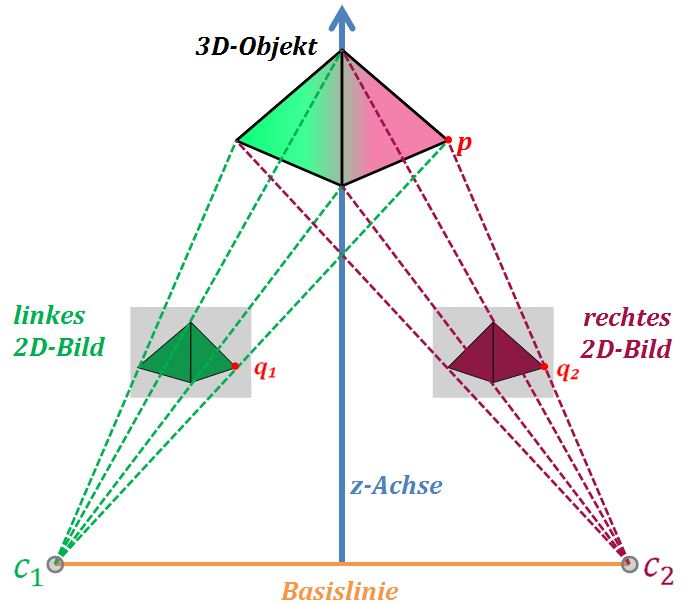
\includegraphics[width=8cm]{chapters/computervision/grafik_7_stereopsis.jpg}
\caption{Stereopsis mit epipolaren Linien.}
\label{fig:7}
\end{figure}
In Abb. \ref{fig:7} ist die Idee der Stereopsis skizziert. $c_1$ stellt die linke Kamera, $c_2$ die rechte dar. Die gestrichelten Linien sind die \textbf{epipolaren Linien}. Damit können wir feststellen, welche zwei Pixel $q_1$ und $q_2$ aus den beiden variierenden 2D-Bildern den gleichen Punkt $p$ des Original-Objektes aus der 3D-Welt darstellen. Pixel, die den gleichen Punkt des Objektes darstellen, müssen immer auf epipolaren Linien der 2D-Bilder liegen. Hierbei besteht
\marginpar[Links]{\small{Notiz: \\Algorithmus von Belhumeur}}
\begin{itemize}
\item \textbf{Eindeutigkeit} (es kann immer nur maximal - denn manchmal wird der Objekt-Punkt wegen Überdeckungen nur von einem Sichtfeld aufgenommen - einen Pixel $q_1$ des einen Bildes zugehörig zu einem Pixel $q_2$ des anderen geben) und
\item \textbf{stückweise Stetigkeit} (abgesehen von Objektkanten und Überdeckungen, haben benachbarte Punkte immer ähnliche Werte).
\end{itemize}

\item Textur

Die Textur von Oberflächen in der Welt ist ein sich wiederholendes invariables Muster. Im Bild wird dies durch \textit{texel} (\textbf{tex}ture \textbf{el}ements) repräsentiert, welche in ihrer Grö"se und Gestalt aufgrund der texel-Richtung (Verkürzung falls nicht orthogonal) relativ zur Kamera sowie auch durch unterschiedlichen Abstand zur Kamera sehr stark variieren können.

\marginpar[Links]{\small{Notiz: \\Algorithmus von Malik und Rosenholtz}}
Mit Hilfe von \textbf{texture-Gradienten}, Funktionen der Oberflächengestalt unter Berücksichtigung der Textur-Abschrägung und -Neigung, kann die Veränderungsrate von Bereich, Verkürzung und Dichte der texel aufgeklärt werden.

\item Kontur

Konturen sind Linien, welche verschiedene Bedeutungen haben können, die wir ihnen zuordnen möchten. Hierfür betrachten wir einfache Strichzeichnungen und unterscheiden zunächst zwei grobe Klassen, welche wir anschlie"send verfeinern:

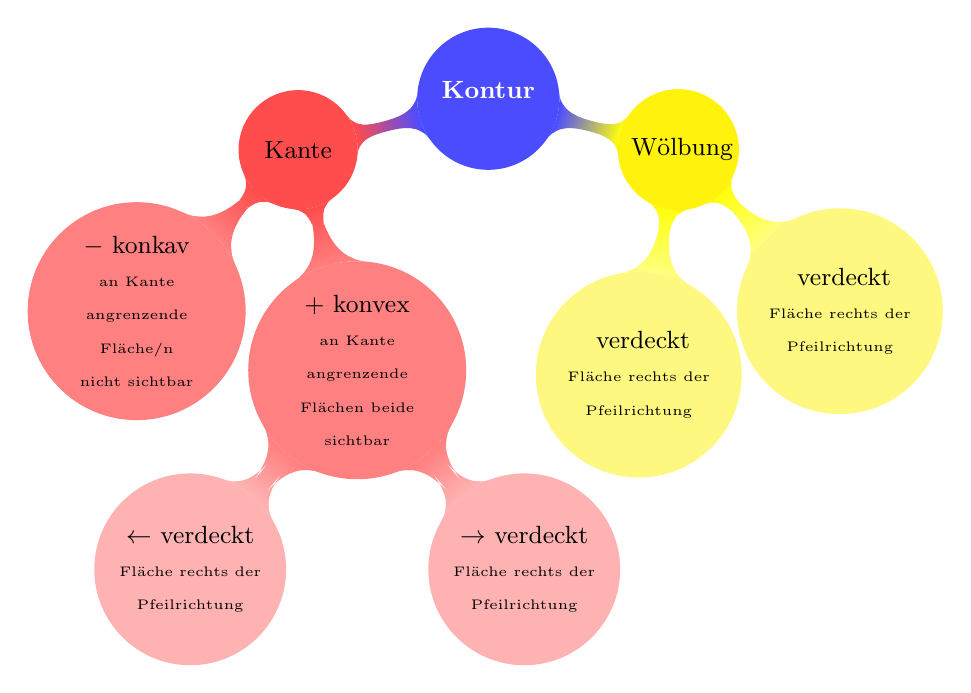
\begin{tikzpicture}[grow cyclic, text width=1.2cm, align=flush center, every node/.style=concept, concept color=blue!70, text=white,
level 1/.style={level distance=2.5cm,sibling angle=130},
level 2/.style={level distance=2.9cm,sibling angle=60},
level 3/.style={level distance=3.3cm,sibling angle=85}],

\node {\textbf{ \small{Kontur} } } [text=black, clockwise from=-35]  % root node
   child [concept color=yellow!95, grow=-15] { node  {\small{Wölbung}} [clockwise from=-45]
     child [concept color=yellow!50] { node [text width=2cm] {
     	\small{$\twoheadleftarrow$ verdeckt}\\\tiny{Fläche rechts der Pfeilrichtung}}}
     child [concept color=yellow!50, grow=-100] { node [text width=2cm] {
     	\small{$\twoheadrightarrow$ verdeckt}\\\tiny{Fläche rechts der Pfeilrichtung}}}
    }
   child [concept color=red!70] { node {\small{Kante}} [clockwise from=-75]
     child [concept color=red!50] {
     node [text width=1.5cm] {
     \small{$+$ konvex}\\\tiny{an Kante angrenzende Flächen beide sichtbar}}
          child [concept color=red!30, text width=1.5cm, grow=-130] {
         	 node [text width=1.8cm] {
          	\small{$\leftarrow$ verdeckt}\\\tiny{Fläche rechts der Pfeilrichtung}}}
          child [concept color=red!30, text width=1.5cm, grow=-50] {
          	node [text width=1.8cm, minimum width=1.8cm] {
         	\small{$\rightarrow$ verdeckt}\\\tiny{Fläche rechts der Pfeilrichtung}}}
     }
     child [concept color=red!50, grow=-135] {
     node [text width=1.5cm] {
     \small{$-$ konkav}\\\tiny{an Kante angrenzende Fläche/n nicht sichtbar}}
     }
    }    ;
\end{tikzpicture}

So können wir Konturen bspw. klassifizieren:
\begin{figure}[h]
\centering
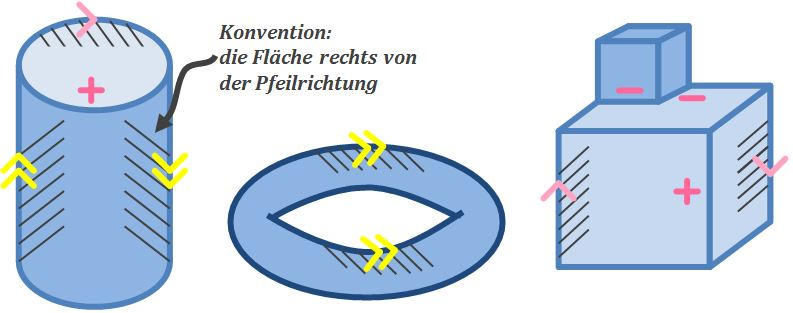
\includegraphics[width=8cm]{chapters/computervision/grafik_8_kontur.jpg}
\caption{Konturklassifizierung.}
\label{fig:8}
\end{figure}

Huffman und Clowes haben unabhängig voneinander ein Schema entwickelt, um systematisch vielgestaltige Bilder zu analysieren. Es werden hierbei Objekte mit bis zu drei aneinandergrenzenden Flächen (Spalten werden ausgeschlossen) pro Eckpunkt betrachtet.
\marginpar[Links]{\small{Notiz: \\Waltz hat einen Algorithmus entworfen, der Spalten, Schatten und getrennte Aushöhlungen berücksichtigt.
Mackworth und Sugihara haben die Linienklassifizierung nach Huffman-Clowes-Waltz für beliebig-flächige Objekte ausgearbeitet.}}
So ergeben sich vier Fälle, wie ein solcher dreiflächiger Eckpunkt entstehen kann:
\begin{figure}[h]
\centering
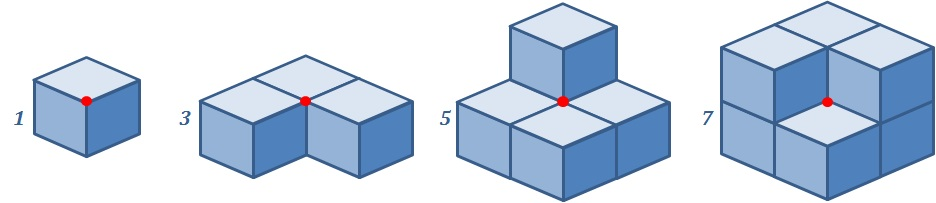
\includegraphics[width=8cm]{chapters/computervision/grafik_9_de.jpg}
\caption{Anordnungen von Würfeln für die Entstehung eines neuen dreiflächigen Eckpunkts (roter Punkt). Die Zahl gibt die Würfelanzahl an.}
\label{fig:9}
\end{figure}

Aus den verschiedenen Sichtweisen der Eckpunkte ergeben sich folgende Konturklassifizierungen:
\begin{figure}[h]
\centering
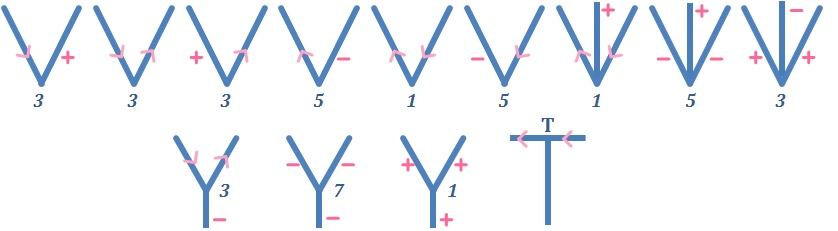
\includegraphics[width=10cm]{chapters/computervision/grafik_10_label.jpg}
\caption{Das Huffman-Clowes Klassifizierungs-Set.}
\label{fig:10}
\end{figure}
\end{itemize}
\section{Objekterkennung: Probleme \& Anwendung}

% Abgrenzung / Vergleich zu den vorherigen Kapitel wo möglich und sinnvoll

\subsection{Probleme}

Menschen ist es möglich, unzählige Objekte zu erkennen, selbst wenn diese teilweise verdeckt oder nur karikiert sind. Für einen Computer ist das nicht so einfach. Er muss über ein gro"ses Reportoire von Objektarten sowie ihre Variationen verfügen und diese dann auch noch im Bild wiederfinden. Dieses Problem der \textbf{Objektvielfalt} können wir für abgewandelte Grundformen wie z. B. Würfel und Zylinder ganz gut lösen: Ein \textbf{verallgemeinerter Zylinder} \label{Zylinder} hat
\begin{itemize}
\item einen ebenen Querschnitt,
\item eine Achse (gerade oder gewölbt) und
\item eine Regel, die die Änderung des Querschnitts entlang der Achse beschreibt.
\end{itemize}
Viele Objekte können in Zylinder zerlegt und somit erkannt werden. Dies kann aber auch dazu führen, dass das Objekt in so viele Zylinder-Teile gebrochen wird, dass sich dies auf die Laufzeit auswirkt.

\subsection{Anwendung}
Betrachten wir eines der am Anfang genannten Hauptanwendungsgebiete der Computer Vision, die Navigation - speziell: automatisiertes Fahren. Die Aufgaben eines Fahrers sind
\begin{enumerate}
\item Beschleunigung des Fahrzeugs,
\item Kontrolle: seitlich (Fahrspur) und längs (Sicherheitsabstand),
\item Wachsamkeit: Verkehrsüberblick und ständige Handlungsbereitschaft.
\end{enumerate}
Nehmen wir Punkt 2 heraus: Welchen Ansatz aus den bisherigen Kapitel könnten wir hier verwenden?

Bei der Kontrolle eines Fahrzeugs gibt es zwei wichtige Bedingungen: Zum einen möchten wir eine Linie bzw. Kante - die Fahrspur - finden und zum anderen möchten wir vor uns liegende Objekte - Autos/Hindernisse - erkennen. Folgende Tabelle zeigt auf, was wir aus dem bisher Gelernten nun anwenden können:
\begin{table}[h]
\centering
\label{Tab. 3.2}
\begin{tabular}{@{}lll@{}}
\toprule
\multicolumn{1}{c}{\textbf{Aufgabe}} & \multicolumn{1}{c}{\textbf{benötigte Infos}} & \multicolumn{1}{c}{\textbf{Ansatz CV}} \\ \midrule
Kontrolle seitlich & Spur, Fahrzeugsposition & Kantenerkennung \\
Kontrolle längst & Distanz zu Objekten & Zweifach-Tiefenwahrnehmung, \\&&Bewegungsfluss \\ \bottomrule
\end{tabular}
\end{table}

Was aber ist mit speziellen Objekten, wie zum Beispiel Verkehrsschilder oder Menschen? Bisher haben wir sozusagen nur die Basis der Objekterkennung kennengelernt - im Folgenden lernen wir noch zwei Methoden zur detailliertere Objekterkennung kennen.

\subsubsection{Abgleichungsmethode}

Wir möchten die Projektion eines 3D-Objektes der Welt auf unserem Bild identifizieren, ohne dass wir die Gestalt, Position und Richtung des Objektes kennen. Wir wissen nur, dass es eine \textbf{skalierte orthografische Projektion} ist, sprich das Objekt wird auf dem Bild nach hinten hin nicht kleiner.
Huttenlocher und \mbox{Ullmann} haben folgende Vorgehensweise (hier vereinfacht) verifiziert:

\begin{enumerate}
\item Wir verfügen über $m$ \textbf{charakterisierende Originalpunkte} \mbox{$\mu_1,\mu_2,...,\mu_m$} des 3D-Objektes in seiner Grundhaltung aus der Welt.
\item Durch Rotation und Verschiebung des 3D-Objekts sowie anschlie"sender Projektion, sodass ein Bild entsteht, verändern sich die Originalpunkte zu $n$ \textbf{charakterisierenden Bildpunkten} $p_1,...,p_n$. \\
Hierbei ist normalerweise $m\neq n$, da Originalpunkte verdeckt werden und nicht/fälschlicherweise (wegen Rauschen) identifiziert werden. (Abb. 3.1)
\begin{figure}[h]
\centering
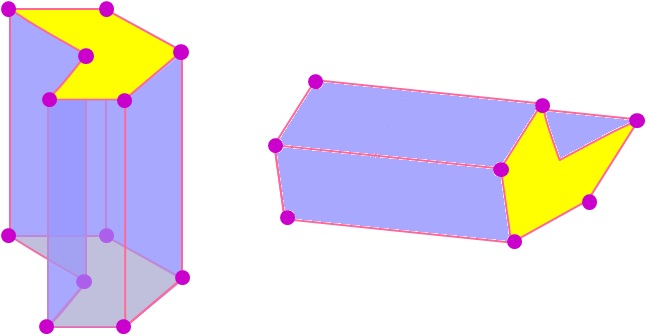
\includegraphics[width=5cm]{chapters/computervision/grafik_14_3d2d.jpg}
\caption{Links: Original 3D-Objekt mit 12 charakterisierenden Punkten. Rechts: 2D-Projektion, nur 8 der Charakterpunkte sind erhalten geblieben.}
\label{fig:14}
\end{figure}

\item $Q$, die unbekannte Rotation und Verschiebung des Objektes, \textbf{transformiert} jedes $\mu_i$ und kreiiert exakt zugehörige Bildpunkte $p_i=Q(\mu_i)$.
\item Wenn wir genug Punkte haben, können wir $Q$ auflösen. Es gilt: Mit drei nonkollinear (nicht auf einer Linie liegenden) Originalpunkten und drei Bildpunkten ergeben sich genau zwei Transformationen des 3D-Objekts.
\begin{figure}[h]
\centering
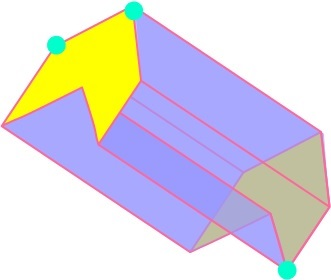
\includegraphics[width=3cm]{chapters/computervision/grafik_13_fixpunkte.jpg}
\caption{Bei drei Fixpunkten (türkis) kann das Objekt nicht rotieren.}
\label{fig:13}
\end{figure}
\end{enumerate}
Man sucht sozusagen eine Funktion, mit der ein Originalpunkt zu einem Bildpunkt transformiert wird: $Q(\mu_i)=p_i$.

Der Algorithmus \textsc{Align} verwendet eine $"$Ausprobier$"$-Lösungsstrategie: \textsc{Align} vermutet zu Originalpunkten zugehörige Bildpunkte und gibt entweder \verb+false+ zurück, falls die Annahme falsch war, oder $Q$, falls sie richtig war.
\begin{figure}[h]
\centering
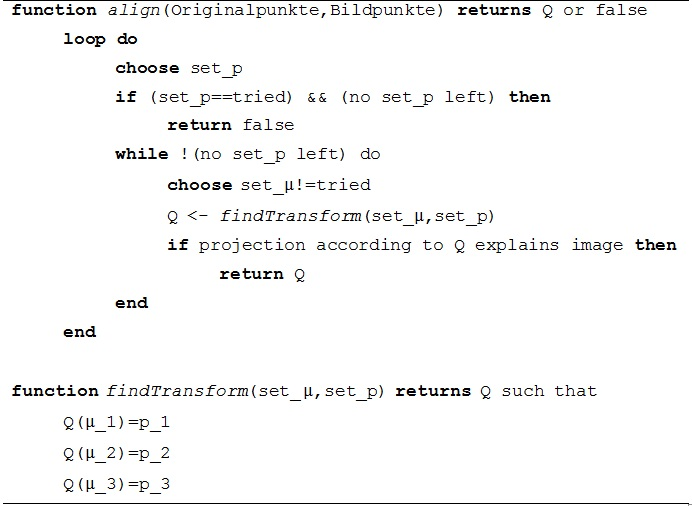
\includegraphics[width=10cm]{chapters/computervision/grafik_15_align.jpg}
\caption{Pseudocode \textsc{Align}.}
\label{fig:15}
\end{figure}

Wir können uns das in etwa so vorstellen:
\begin{itemize}
\item Beispiel:

Wir haben je fünf charakterisierende Punkte unseres 3D- und 2D-Objektes.
\begin{figure}[h]
\centering
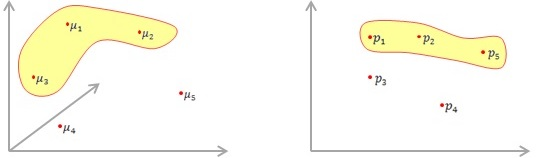
\includegraphics[width=8cm]{chapters/computervision/grafik_11_set.jpg}
\caption{\textsc{Align} ratet ein Set $S_\mu$ von drei Originalpunkten und ein Set $S_p$ von drei Bildpunkten.}
\label{fig:11}
\end{figure}

Jetzt möchten wir eine Transformation $Q$ berechnen. \textsc{Align} $"$ratet$"$ hierfür Paare $(\mu_i,p_j)$ mit $\mu_i\in S_\mu$, $p_j\in S_p$ und $i,j\in\{1,...,5\}$. In unserem Beispiel legt \textsc{Align} die Paare $(\mu_1,p_1), (\mu_2,p_2), (\mu_3,p_3)$ fest.

Wir können uns die Rechnung wie folgt vorstellen, die für jedes Paar angewandt wird:
\begin{figure}[h]
\centering
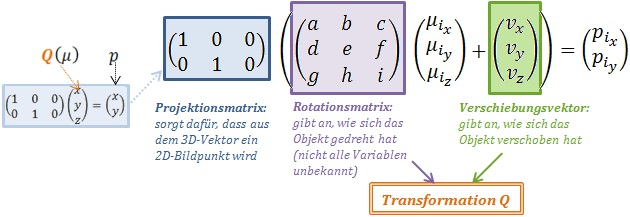
\includegraphics[width=12cm]{chapters/computervision/grafik_12_q.jpg}
\caption{Berechnung der Transformation $Q$.}
\label{fig:12}
\end{figure}

Die gefundene Transformation $Q$ wird nun auf die restlichen, \textit{nicht} im Set vorhandenen Paare - in unserem Beispiel bleiben die Kombinationen $(\mu_4,p_4), (\mu_5,p_5), (\mu_4,p_5), (\mu_5,p_4)$ - angewandt. Wenn für ein Paar, bei dem \textsc{Align} $Q$ auf $\mu$ anwendet, genau das Ergebnis $p$ rauskommt, dann haben wir die richtige Transformation $Q$ gefunden. Falls nicht, werden zwei neue, noch ungetestete Sets ausgewählt und es geht von vorne los.
\item Laufzeit

Im schlimmsten Fall liegt die Laufzeit in $O(m^4n^3log$ $n)$, denn $Q$ muss so oft berechnet werden, wie es Sets gibt, das ist $\binom{m}{3}\binom{n}{3}$ und die Überprüfung von $Q$ kostet nochmal $m$ $log$ $n$.

Olson hat die Laufzeit auf $O(mn^3)$ wie folgt verbessert:
\begin{itemize}
\item $"$pose-clustering$"$: Er \textbf{gruppiert} nur sich ähnelnde - somit nah an der korrekten Transformation liegende - $Q$-Transformationen, was in $O(mn)$ liegt.
\item Wenn wir im Vorhinein zwei Paare $(\mu_1,p_1)$ und $(\mu_2,p_2)$ gegeben hätten, könnten wir das Set komplettieren, indem wir das dritte Paar aus den Schnittpunkten der verlängerten Linien ablesen (Abb. \ref{fig:16}).
Olsen nutzt dieses Prinzip mit der \textbf{randomisierten} Auswahl zweier Paare, das kostet $O(n^2)$.
\begin{figure}[h]
\centering
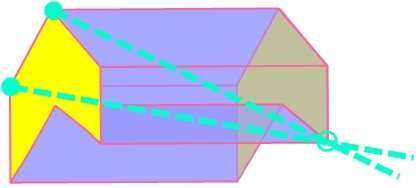
\includegraphics[width=4cm]{chapters/computervision/grafik_16_line.jpg}
\caption{Geometrische Berechnung des dritten Punkts aus zwei gegebenen Punkten.}
\label{fig:16}
\end{figure}
\end{itemize}

\subsubsection{Projektive Invarianz}

Hier haben wir eine Bibliothek mit verschiedenen Objekten.
Jedes Objekt hat einen \textbf{invarianten Wert} ($"$index function$"$) $I$, welcher mit Hilfe der geometrischen Invarianz als Repräsentation für alle Posen, die das Objekt annehmen kann, erstellt wird (Abb. \ref{fig:17}).
\begin{figure}[h]
\centering
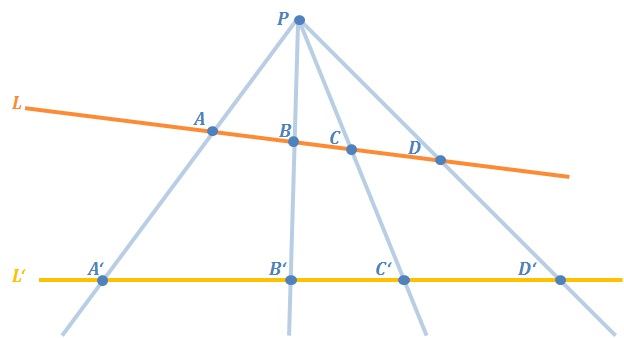
\includegraphics[width=6cm]{chapters/computervision/grafik_17_invar.jpg}
\caption{Ein einfaches Beispiel für die projektive Invarianz: Doppelverhältnis von vier Punkten auf einer Geraden. Solange $L$ nicht durch $P$ geht, gilt: $(A,B;C,D)=\frac{AC\cdot BD}{BC\cdot AD}=\frac{A'C'\cdot B'D'}{B'C'\cdot A'D'}=(A',B';C',D')$}
\label{fig:17}
\end{figure}

Ein Objekt wird als Modell mit seinen charakterisierenden Eigenschaften abgespeichert (diese sind u. a. Name, Kanten, Kegelquerschnitte
\marginpar[Links]{\small{Notiz:\\Wir erinnern uns an \ref{Zylinder}: Objekte können in Zylinder zerlegt werden - Zylinderquerschnitte sind \textit{Kegelquerschnitte}}}
, Wölbungen, $I$).
Die Aufnahme von Modellen ist sehr einfach, sie kann zum Beispiel direkt von einem Bild - ohne spezielle Kenntnisse über die Kameraposition etc. - übernommen werden.

Zusätzlich generiert jedes $I$ seine eigene Hypothese. Die $I$s sind idealerweise alle einzigartig - falls sehr viele Objekte in der Bibliothek sind, ist das manchmal nicht möglich, dann werden sie zu einer gemeinsame Hypothese für diese Objekte kombiniert.

Die Objekterkennung geschieht dann wie folgt:
\begin{enumerate}
\item Kanten finden und bündeln
\item $I$ messen
\item Nach Übereinstimmung in Bibliothek suchen:
\begin{table}[h]
\centering
\begin{tabular}{lll}
entweder & $I$ gefunden und einzigartig & $\Rightarrow$ Objekt erkannt \\
oder & $I$ ist nicht einzigartig $\rightsquigarrow$ Hypothese des Modells mit &  \\
 & grö"sten Übereinstimmung (i. A. ab 50\%) wird bestätigt & $\Rightarrow$ Objekt erkannt \\
oder & $I$ nicht gefunden & $\Rightarrow$ Objekt \textit{nicht} erkannt
\end{tabular}
\end{table}
\end{enumerate}
Anwendung findet diese Methode beispielsweise bei Satellitenaufnahmen.
\end{itemize}

\section{Fazit \& Bewertung}

Computervision ist die Königsdisziplin der Informationsverarbeitung. Was bei uns Menschen automatisch passiert ist für eine KI nur mit raffinierten Berechnungen annähernd möglich.

Bspw. ist die effektive Repräsentation von Objektarten - vorallem für gewölbte Objekte - grö"stenteils noch ungelöst. Es ist nicht nur aus wissenschaftlicher Sicht interessant sondern auch aus industrieller: würden wir mehr darüber wissen, könnten wir z. B. den Robotern besser beibringen, wie sie Objekte erkennen, greifen, bearbeiten, und so weiter.

In den letzten Jahrzehnten hat sich zwar viel getan (z. B. ist jede Digitalkamera heutzutage standardmä"sig mit einer Gesichtserkennung ausgestattet, sind automatische Fahr- und Bremssysteme von Automobilherstellern bereits auf dem Markt, ...), dennoch ist der Mensch unverzichtbar: er wird dort gebraucht, wo die Maschine (noch) an ihre Grenzen stö"st.

\section{Weitere Anwendungsgebiete}
Die Hauptanwendungsgebiete neben der \textbf{Objekterkennung} sind \textbf{Manipulation} der dreiminesionalen Welt und \textbf{Navigation} (Pfaderkennung, Ausweichmanöver, etc.). Diese und andere Einsatzgebiete neben den zur Veranschaulichung schon bereits besprochenen Nutzungsmöglichkeiten der Objekterkennung werden in den folgenden Abschnitten dargelegt.


\subsection{Bilder und Schlagworte}
Heutzutage bietet das Internet die Möglichkeit, anhand von Schlagwörtern nicht nur nach Text zu suchen, sondern auch Bilder zu finden. Das automatisierte Versehen von Bilder mit Schlagworten ist sehr wichtig: Wir haben eine Menge von Beispielbildern und möchten mit diesen einige Testbilder abgleichen (\textbf{Problem der Auto-Annotation}). Das beste Ergebnis erhält man mit der \textbf{Nächste-Nachbarn-Klassifikation}, die die Trainingsbilder raussucht, die dem Testbild durch bestimmte Merkmalsausprägungen am ähnlichsten sind. Die Schwierigkeit liegt in der Erkennung von Aktionsmustern. Man kann zwar schon durch Hintergrundsubtraktion und anschließeneder Betrachtung von HOG-Merkmalen basierend auf dem optischen Fluss die Verhaltensstrukturen annährend gut erkennen und so beispielsweise einen trinkenden Menschen im Bild ausfindig machen (Hand wird mit Objekt zum Mund geführt), allerdings ist diese Erkennung sehr eingeschränkt: Man könnte mit diesen Merkmalsausprägungen keine trinkende Katze in einem Bild erkennen.


\subsection{Rekonstruktion}
Besteht die Vermutung, was für ein Objekt sich auf einem Testbild befindet, so reicht manchmal allein schon dieses Bild aus, um mehrere Ansichten des Objekts zu erstellen. Wenn das Objektmodell, d.h. die Repräsentation des Objekts in dem Klassifizierer, aus mehreren Punkten oder sogar Bildern besteht, können wir Korrespondenzen zu Punkten aus dem Testbild dokumentieren. Anhand der Punkte können wir dann die Parameter der Kamera, falls diese nicht vorliegen, bestimmen und überprüfen, ob die Modellpunkte mit den Bildpunkten übereinstimmen.

Diese Technologie der Rekonstruktion ist heutzutage so hochentwickelt, dass sie in folgenden Bereichen zur Anwendung kommt:
\begin{itemize}
  \item \textbf{Modellerstellung} (z.B. dreidimensionale Karten)
  \item \textbf{Bewegungsabgleich} (z.B. bei animierte Figuren in realen Filmsequenzen)
  \item \textbf{Pfadrekonstruktion} (z.B. bei mobilen Robotern)
\end{itemize}


\subsection{Bewegungssteuerung}
Wie wichtig die Manipulation von Objekten und die Navigation beispielweise beim Ausweichen von Hindernissen ist, wird nicht nur in der Tierwelt deutlich. Wollen wir ein Visionssystem für ein \textbf{selbstfahrendes Fahrzeug} implementieren, so hat dies für folgende Aufgaben geeignete Aktionen zu finden:
\begin{itemize}
  \item \textbf{Seitensteuerung}: innerhalb der Spur bleiben oder Spurwechsel ausführen.
  \item \textbf{Längssteuerung}: bremsen, beschleunigen, Abstand halten.
  \item \textbf{Ausweichen}: Objekte in der Nähe beobachten und Kollisionen vermeiden.
\end{itemize}
Für die Seitensteuerung werden Algorithmen zur Kantenerkennung: Sie dienen dazu, Mittelstreifen zu erkennen und die Position und Ausrichtung des Autos relativ zur Spur zu verwalten.\\
Für die Längssteuerung und das Wahrnehmen von Hindernissen müssen wir Abstandserkennung mit Strukturerkennung kombinieren: Durch binokulares Stereosehen oder durch optischen Fluss, unterstützt durch HOG-Merkmale, können sich Fahrzeuge an Verkehrsregeln halten.

Mobile Roboter stellen eine größere Herausforderung da. Eine Methode zur Lokalisierung dieser in ihrer Umgebung besteht aus stereoskopischen Kamerasystemen. Um bei schlechten Lichtverhältnissen mit genügend Informationen versorgt zu werden, ist von den zwei Systemen eins nach vorne und das andere nach hinten ausgerichtet. Sollte die Beleuchtung allerdings doch mal erheblich schlecht sein, sorgt ein Trägheitsmodul, das ähnlich wie unser Gleichgewichtsorgan funktioniert, für die weitere Informationsbereitstellung.

Ein weiteres Problem der (visuellen) \textbf{Odometrie} (Bestimmung der Positionsänderung) ist die "`Drift"', bei der sich kleine Positionsabweichungen mit der Zeit aufaddieren. Zur Lösung dieses Problems werden feste Standpunkte in der Umgebung installiert, an denen der Roboter sich orientieren kann.

\section{Quellen und Literatur}
Die Ausarbeitung stützt sich hauptsächlich auf das Buch
\begin{enumerate}
\item []
Artificial Intelligence - A Modern Approach \\
von Stuart J. Russell and Peter Norvig (1995, Kap. 24.2.4 aus 2016)
\end{enumerate}
Weiteres habe ich hier nachgelesen:
\begin{enumerate}
\item [] http://aima.cs.berkeley.edu/
\item [] http://faculty.washington.edu/cfolson/papers/pdf/ijcv97.pdf
\item [] Object Representation in Computer Vision II\\ von Jean Ponce, Andrew Zisserman, Martial Hebert
\item [] http://e-collection.library.ethz.ch/eserv/eth:25629/eth-25629-03.pdf
\item [] https://www-m10.ma.tum.de/foswiki/pub/Lehre/WS0809/\\GeometrieKalkueleWS0809/GeoKalkSkript.pdf
\item [] www.wikipedia.de
\item [] https://www.bmvi.de/SharedDocs/DE/Anlage/Digitales/bericht-zum-forschungsbedarf-runder-tisch-automatisiertes-fahren.pdf?\_\_blob=publicationFile (2015)
\item [] http://tex.stackexchange.com/questions/232550/visual-table-of-contents-using-tikz-mindmap-or-similar
\item [] http://www.texample.net/tikz/examples/servers/
\end{enumerate}
